
% SEP 2012 Group 13
% Software Design Document (SDD)
%
\documentclass[11pt, a4paper]{report}
\usepackage{graphicx}
\usepackage{fullpage}
\usepackage{url}
\pagestyle{headings}

%%% page parameters
\headsep = 25pt
\begin{document}
\oddsidemargin -0.5 cm
\evensidemargin -0.5 cm
\textwidth 15 cm
\topmargin -1.2 cm
\textheight 25 cm
\begin{center}

\includegraphics[scale=1.5]{./UniLogo}\\[1cm]    
\textbf{\Huge \bfseries Software Design Document}\\[1.5cm]
\textbf{\huge for}\\[0.5cm]


% Title
\textbf{ \huge Archaeology Robot }\\[0.3cm]
\textbf{ \huge Group 13 }\\[2cm]


\begin{tabular}{ |c | p{2cm} |}
	\hline
Yufeng Bai 1600095 & \\[.5cm] \hline
Dawei Geng 1219181 & \\[.5cm] \hline
Jun Chen 1206265 & \\[.5cm] \hline
Quang Khoi Nguyen 1187070  & \\[.5cm] \hline
Shikai Li 1214223 & \\[.5cm] \hline
Yunyao Yao 1203525 & \\[.5cm] \hline
Yatong Zhou 1204471 & \\[.5cm] \hline
\end{tabular}


\vfill

% Bottom of the page
Version 1.31 \\ [0.2cm]
{\large \today}

\end{center}
\tableofcontents



% Version History %

% IMPORTANT %
% Whenever you make a change to this document you MUST put an entry in below
% Must conform to firstName lastName &  date & discription \\ \hline


\clearpage
\section*{Revision History}
\begin{tabular}{| l | l | l | l | }
\hline
Name      		&	Date        	&	Reason For Changes                  	  	&	Version     	\\ \hline
Dawei Geng      &	03 Sep 2012     &	Template			                  	  	&	0.1 	    	\\ \hline
Yufeng Bai         &	06 Sep 2012	&	Chapter 7						&	0.2		\\ \hline
Yufeng Bai	&	06 Sep 2012	&	Chapter 8						&	0.3		\\ \hline
Yufeng Bai	&	06 Sep 2012	&	Chapter 9						&	0.4		\\ \hline
Yufeng Bai	&	07 Sep 2012	&	Fix the layout					&	0.5		\\ \hline
Jun Chen    &   08 Sep 2012 &	Chapter 1                  	  	&	0.6     	\\ \hline
Jun Chen   	&	08 Sep 2012 &	Chapter 2                 	  	&	0.7     	\\ \hline
%Name      		&	Date        	&	Reason For Changes                  	  	&	Version     	\\ \hline
%Name      		&	Date        	&	Reason For Changes                  	  	&	Version     	\\ \hline
%Name      		&	Date        	&	Reason For Changes                  	  	&	Version     	\\ \hline
%Name      		&	Date        	&	Reason For Changes                  	  	&	Version     	\\ \hline
%Name      		&	Date        	&	Reason For Changes                  	  	&	Version     	\\ \hline
%Name      		&	Date        	&	Reason For Changes                  	  	&	Version     	\\ \hline
%Name      		&	Date        	&	Reason For Changes                  	  	&	Version     	\\ \hline
%Name      		&	Date        	&	Reason For Changes                  	  	&	Version     	\\ \hline
%Name      		&	Date        	&	Reason For Changes                  	  	&	Version     	\\ \hline






\end{tabular}
\clearpage

% Introduction %

\chapter{Introduction}% (fold)
\label{cha:I}
%Provide an overview of the SDD and a description of the scope of the system to be developed.%


\section{Purpose and Scope}
\subsection{Purpose}
The purpose of making this Software Design Document (SDD) is to give the details of the design of the archaeology robot and its system, which is designed by our group (group 13). In this document, we will give an overall description of architectural design, system organisation and critical modules of the system. This document describes some general ideas of how do we design the system and how do we implement requirements into the system. This document will be given to the team members so that they can construct the system based on the requirements. Also this document will be used as a reference for further developments.
%Define the purpose of this document, specify intended readership of the docu- ment.%


\subsection{Scope}
This Software Design Document (SDD) is to give details  of overall design of archaeology robot. It will contain nine parts : Introduction which will give an overall description of the design, System Overview which will show the design of the system, System Architecture and Components Design, Architectural Description which also includes alternatives and rationale, Data Design, Human Interface Design, Resource Estimates and Definitions, Acronyms and Abbreviations. 
%Identify the context of the system; explain what the proposed system does (and what does not, if necessary); describe the relevant benefits, objectives and goals. The description should be consistent with your SRS.%


\section{References}
This Software Design Document (SDD) references these files below:
\newline
\item Software Requirements Document (SRS) : this document demonstrate all the requirements for this project.
\newline
\item Software Project Management Plan (SPMP) : this document shows the details of how do we manage our project.
\newline
\item UML files : the class diagram show how do we design and implement our system.
\newline
%Provide a complete list of all documents that you referenced in SDD.%


\section{Overview}
This Software Design Document will be organized in a way that describe System, Architectural Design, GUI Design and Resource Estimates logically. In the beginning of the document, it will give an introduction of this document (Purpose and Scope) and System Overview. After that, the document will give some high level architectural design of the whole system, which include System Architecture and Components Design, Architectural Description. Then the document will move to the Data Design, which also includes Design Details. After the Data Design, it will also shows the design of Human Interface and Resource Estimates. Lastly, there are some Definitions, Acronyms and Abbreviations at the end of the document. This document will follow the developing stages.
%Overview the content of the document; explain how the SDD is organized.%

\section{Constraints}
The follow restrictions, limitations, and constraints will affect the design and implementation of the system:
\begin{itemize}
  \item The robot should be set up correctly before testing.
  \item The robt can not be damaged.
  \item The robt can not wlak out of map.
  \item The robt can not push the wall and colliding is not permitted.
  \item The map should be set up correctly before testing
  \item The map is in fixed size (less than A1)
  \item There are some no-go zone on the map.
  \item The system must has save and load function.
  \item An acceptable latency is 300ms.
  \item There are some hidden wall in the map.
\end{itemize}
%Briefly describe any restrictions, limitations, and constraints that affect the design and implementation of the system.%


% chapter Introduction (end)
\pagebreak


\chapter{System Overview}% (fold)
\label{cha:SO}
The main goal of the system is to let the robot can be used for survey an archaeological site containing the remnants of an ancient city on the premise that the robot can not be damaged.
\newline
\newline
 Firstly, the system of the robot will use light sensor, touch sensor and ultrasonic sensor to locate some objects on the map, which include:
\begin{itemize}
  \item walls
  \item hidden walls 
  \item obstacles on the surface
\end{itemize}
Secondly, the robot which is used to survey an archaeological site is programmed by leJOS software. With this softeware we can design the functionalities of the robot correctly, so that it can detect every object on the map on the premise that the robot is not damaged. When the robot detect somethings, the system should deal with it by using a proper way which is described in the Sofeware Requirements Document (SRS).
\newline
\newline
Thirdly, the operating sofeware of the robot will have a nice graphic user interface (GUI) which contains:
\begin{itemize}
  \item Control panel
  \item Map area
  \item robot information
  \item battery usage
  \item mode
  \item etc..
\end{itemize}
Lastly, the database of this project shall contain XML map files to store and update the survey map, the map shows :
\begin{itemize}
  \item the whole map
  \item No-go zone
  \item detected walls
  \item detected hidden wall
  \item detected obstacles
  \item unexplored zone
  \item explored zone
  \item the boundary of the map
  \item initial point
\end{itemize}
\newline
In conclusion, the whole system of this project contains four parts:
\begin{itemize}
  \item Client System which is installed in the robot for implementing its functionalities.
  \item User(Host) System which is used to control the robot and do things the clients want.
  \item GUI System is used to give a graphic user interface to the User System so that it is easier to be used.
  \item Database System which will store the survey result into a XML map.
\end{itemize}
With these four parts the system will work properly and do the task based on the requirements.

%Briefly introduce the system context and design.%


% chapter System Overview (end)
\pagebreak


\chapter{System Architecture and Components Design}% (fold)
\label{cha:SACD}
%In this section, you should cover the following content, in several subsections.%


\chapter{Architectural Description}
%Describe the architectural design of the whole system. Typically, you should include a block diagram showing the major subsystems and their interconnec- tions.%


\section{Component Decomposition Description}
%A decomposition of the subsystems that summarizes the software components.%


\section{Detailed Components Design Description}
%Give the detailed design for each component. In particular, for each component, you need to provide:
%� Component Identifier: An identifier unique to this component.
%� Purpose: A reference (link) back to the requirement specification (SRS).
%� Function: What does this component do? Describe its functionality.
%� Subordinates: The components used by this component.
%� Dependencies: Constraints placed on this component by other compo- nents.
%� Interfaces: Control and data flow in and out of the component.
%� Data: Description of internal data if there is any.


\section{Architectural Alternatives}
%Discuss briefly other architectures that were considered if any.%


\section{Design Rationale}
%Discuss the rationale on selecting the architecture described in 3.1, including the critical issues and tradeoffs that were considered.%


% chapter System Architecture and Components Design (end)
\pagebreak


\chapter{Data Design}% (fold)
\label{cha:DD1}
%You should cover database description and data structures in this section.%


\section{Database Description}
%Describe briefly the database(s) that is part of the system.%


\section{Data Structures}
%Give the detailed design of the database, i.e., entities and their relationships. You can use either ER model or UML for this purpose.%


% chapter Data Design (end)
\pagebreak

\chapter{Design Details}% (fold)
\label{cha:DD2}
%You shall describe your design by using the following diagrams to reflect all the major requirements that you documented in the SRS.%


\section{Class Diagrams}
%Describe all class diagrams that are considered in the system. Give the details (e.g., attributes, operations) associated with the class.%


\section{State Diagrams}
%Present the state diagrams of objects involved.%


\section{Interaction Diagrams}
%Present the interactions of objects involved.%
%Note: all the diagrams shall be numbered and link to the requirements in%
%the SRS; UML notations should be strictly followed.%


% chapter Design Details (end)
\pagebreak


\chapter{Human Interface Design}% (fold)
\label{cha:HID}

\section{Overview of the User Interface}
%Describe briefly the general functionalities of the system from end users� per- spective.%
The Graphical User Interface is used to communicate with the robot. The GUI is connected with robot, the client is able to control the robot by GUI. When the robot finishes its task, the client is allowed to switch off and disconnect with robot. In addition, the GUI demonstrates the status of the robot. The status includes the speed, the power and the location of the robot. The GUI also shows the obstacles, the "no-go" zone and hidden walls, which is able to be checked on the map window.\\

The GUI is able to demonstrate the follow functions for users:
\begin{itemize}
\item Save map to a XML file
\item Load map from a XML file
\item Change the control mode
\item Demonstrate the Bluetooth and Battery status
\item Control the moving direction of the robot(i.e. forward, backward, rotating)
\item Demonstrate the Icon of the map
\item Demonstrate the Log Information
\item Change the speed of the robot
\item Demonstrate the coordinate of the robot
\end{itemize}
The GUI is displayed below:    
\pagebreak
\begin{center}
 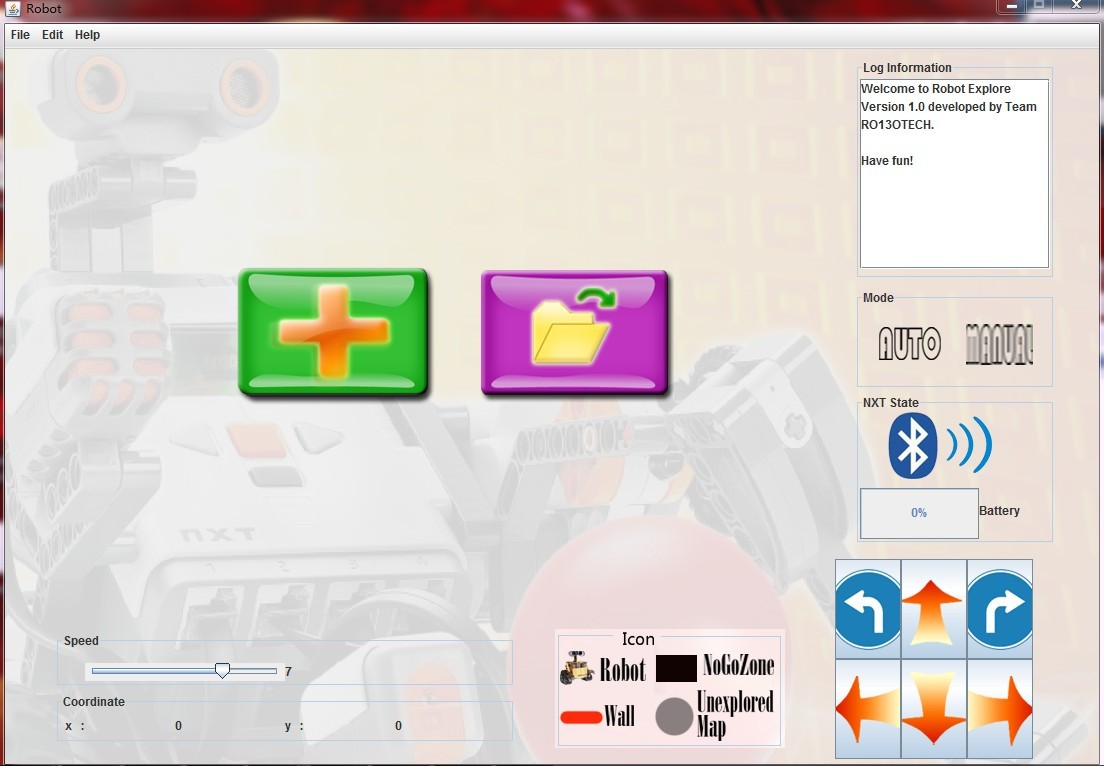
\includegraphics[width=11.20cm]{GUI.jpg}
\end{center}
\begin{center}
\textbf {Figure 11: GUI} \\[0.3cm]
\end{center}
\begin{center}
 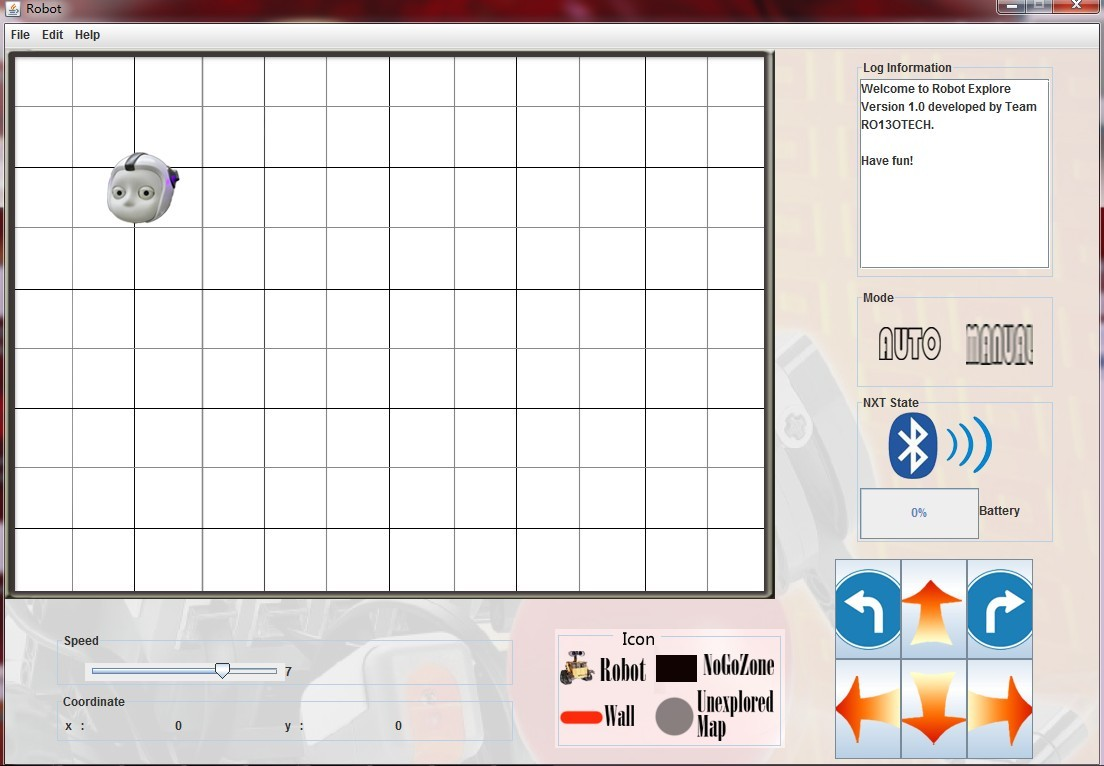
\includegraphics[width=11.20cm]{GUI2.jpg}
\end{center}
\begin{center}
\textbf {Figure 12: GUI WITH MAP} \\[0.3cm]
\end{center}
\section{Deatiled Design of the User Interface}
\subsection{Save map}
The GUI includes a icon which is used to save the map from a XML file. When the client presses the File menu and choose the save option, there is a window jumping out, the client is able to choose the file where the client want to save.  
\begin{center}
 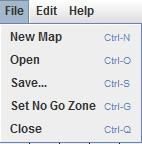
\includegraphics[width=9.20cm]{save}
\end{center}
\begin{center}
\textbf {Figure 13: SAVE MAP} \\[0.3cm]
\end{center}
\subsection{Load map}
The GUI includes a icon which is used to load the map from a XML file. When the client presses that icon, there is a window jumping out, the client is able to choose the map from there. 
\begin{center}
 
\includegraphics[width=9.20cm]{load}
\end{center}
\begin{center}
\textbf {Figure 14: LOAD MAP} \\[0.3cm]
\end{center}
\subsection{Change the control mode}
The client is allowed to change the control mode by pressing the mode button. When the client presses the Auto mode button, there is a widget jumping out. Then if the client presses "yes", the robot changes to the Auto mode. The client is allowed to do the same operation to change to the Manual mode.  The Log information display which mode it is currently.  
\begin{center}
 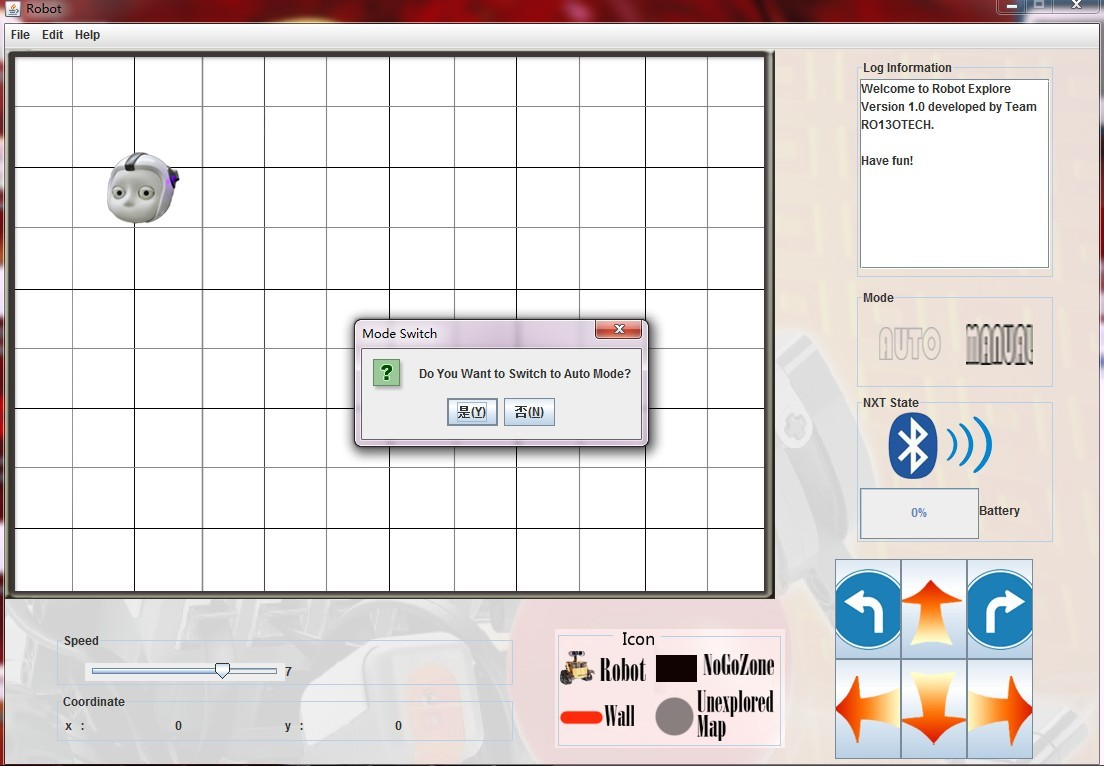
\includegraphics[width=11.20cm]{changemode.jpg}
\end{center}
\begin{center}
\textbf {Figure 15: Change Mode} \\[0.3cm]
\end{center}
\begin{center}
 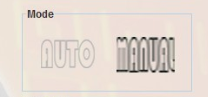
\includegraphics[width=11.20cm]{changemode2}
\end{center}
\begin{center}
\textbf {Figure 16: Change Mode icon} \\[0.3cm]
\end{center}
\subsection{Demonstrate the Bluetooth and battery status}
The Bluetooth and battery status are displayed on the GUI, if the bluetooth loses the connection, the log information board will demonstrate the lose information. The power of the battery is displayed by the percentage number and the colour of the battery bar will change along with the battery level.
 \begin{center}
 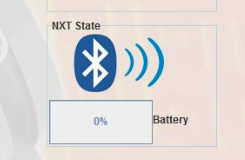
\includegraphics[width=11.20cm]{bluetooth_battery}
\end{center}
\begin{center}
\textbf {Figure 17: Bluetooth and battery demonstration } \\[0.3cm]
\end{center}
\subsection{Control the moving direction of the robot}
The robot is able to be controlled by GUI when the robot is changed to the Manual mode. The client is allowed to press the arrows to move the robot. The robot is able to move forward, backward and rotate(include rotate 90 angles and rotate 360 angles). The moving direction controlling only can be used in Manual mode.
 \begin{center}
 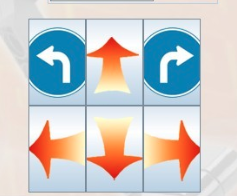
\includegraphics[width=11.20cm]{direction}
\end{center}
\begin{center}
\textbf {Figure 18: Moving control} \\[0.3cm]
\end{center}
\subsection{Demonstrate the icon of the map}
The robot and map information are required to be displayed on the GUI. It is necessary to use different icons to demonstrate the different map information.
  \begin{center}
 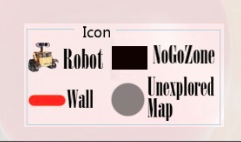
\includegraphics[width=11.20cm]{icon}
\end{center}
\begin{center}
\textbf {Figure 19: Icon of the map} \\[0.3cm]
\end{center}
\subsection{Demonstrate information of the GUI on the log information board}
The Log Information board displays the information of the GUI. For example, the Log Information board demonstrates the version and the developers of the robot. If the client changes the control mode, the board displays which mode it is now. The board also is required to indicate the connection information.
  \begin{center}
 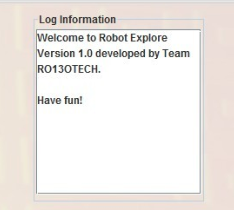
\includegraphics[width=11.20cm]{board}
\end{center}
\begin{center}
\textbf {Figure 20: The logging information} \\[0.3cm]
\end{center}  
\subsection{Control the speed of the robot}
The GUI includes a speed bar and one specific number to control the speed of the robot. The client is allowed to change the speed of the robot by change the number of the bar. The larger number means the faster the robot is. If the number is zero, it means the robot stops immediately.
  \begin{center}
 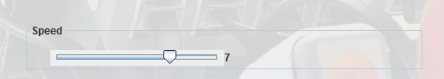
\includegraphics[width=11.20cm]{bar}
\end{center}
\begin{center}
\textbf {Figure 21: The speed controlling} \\[0.3cm]
\end{center}    
\subsection{The location of the robot}
The GUI is required to display the specific location of the robot. The map is made up of a lot of grids. The location of the robot is able to display by coordinate, which is more accurate. When the robot moves, the coordinate will changes immediately.
   \begin{center}
 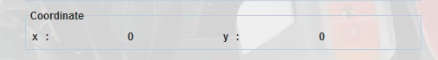
\includegraphics[width=11.20cm]{coordinate}
\end{center}
\begin{center}
\textbf {Figure 22: The coordinate of the robot} \\[0.3cm]
\end{center}        
 
  
%You have to present your user interface design from the following perspectives:
%� Screen Images: screenshots showing the interface from end users� perspec- tive.
%� Screen Objects and Actions: discussion of screen objects and the actions associated with those objects.
%� Report Forms: a description of major reports provided by the system, if any.
%Note: all the interface designs have to link to the user requirements and functional requirements in the SRS; all the interface images shall be num- bered.


% chapter Interface Design (end)
\pagebreak




\chapter{Resource Estimates} % (fold)
\label{cha:RE}
%A summary of computer resource estimates required for operating the system.%
The resource of the project is estimated according to the Project Description and the client's requirements in every week's meeting. All hardware and software which are used in the project are demonstrated below.
\section{Hardware}
\subsection{Robot}
Name: NXT Robot includes all components of the robot\\
Function: The robot is used to search the map and find all the obstacles, hidden walls and "no-go" zone. All operations are required to finish by controlling the robot.
\subsection{Host}
Name: PC\\
Function: The PC is required to demonstrate the searching information of the robot. PC is also used to control the robot on Manual Mode. The programs are uploaded to the robot from the PC.
\subsection{Connection}
Name: Bluetooth and USB \\
Function: The Bluetooth and USB are all used to connect with the robot. The USB is limited by the length of the cable. The bluetooth is limited by the uploading speed. In this project, the USB is used to upload the program and the bluetooth is used to implement the manual control.
\section{Software}
\subsection{Operation Environment} 
Name: Mac, Linux and Windows\\
Function: This project is not providing the working environment. Any system is able to develop the programs for the robot.
\subsection{Developing language}
Name: Java, latex\\
Function: The codes are allowed to write in java language, which is convenient to be read by any developers. The documents are required to write by Latex, then generating the pdf documents.
\subsection{Developing tool}
Name: Eclipse\\
Function: Eclipse is a better tool to make the program for this project. The Eclipse is used to write the operation commands for the robot and draw the GUI for this project.
\subsection{Robot Software}
Name: leJOS 0.9.1\\
 Function: The leJOS is used to control the robot and developing tool is required to support the leJOS 0.9.1. 
 \subsection{Testing tool}
 Name: JUnit\\
 Function: The JUnit is used to debug the code.

% chapter Resource Estimates (end)
\pagebreak

\chapter{Definitions, Acronyms, and Abbreviations} % (fold)
\label{cha:DAA}
\section{Acronyms and Abbreviation}
\begin{center}
\begin{tabular}{|l|c|}
  \hline
  \textbf{Acronyms/Abbreviation} & \textbf{Description}\\
  \hline
  API		& Application Programmable Interface \\
  \hline
  BT		& Bluetooth \\
  \hline
  GUI		& Graphical User Interface \\
  \hline
  PC		& Personal Computer\\
  \hline
  SRS	& Software Requirements Specifications \\
  \hline
  SPMP 	& Software Project Management Plan \\
  \hline
  UML	& Unified Modeling Language\\
  \hline
  USB	& Universal Serial Bus\\
  \hline
  XML 	& eXtensible Markup Language \\
  \hline
\end{tabular} \\[0.3cm]
\textbf {Table 1: Acronyms/Abbreviations} \\[0.3cm]
\end{center}
%Provide definitions of all terms, acronyms, and abbreviations used in SDD.%
\section{Definitions}
\item API: A set of classes and interfaces which are used to make the program for the robot include PC API and lejos API.\\
\newline
\items BT: A device to implement the wireless connection.\\
\newline
\items GUI: A interface which is generated on the PC is used to send the commands to the robot.\\
\newline
\items PC: A device which is used to make the program for the robot and build the GUI.\\
\newline
\items UML: A modelling language is used to build the diagrams for the project.\\
\newline
\items USB: A device to implement the wired connection.\\
\newline
\items XML: The data structure is used to store the map information.\\ 
% chapter Definitions, Acronyms, and Abbreviations (end)
\pagebreak
% Appendicies %
\newpage
\appendix

\pagebreak

\chapter{}






\end{document}
